\section{About} 
TGA is a program solving life and death problems in Go ( for more information about Go see~\cite{web:senseis_library} ).
Program is designed to solve problems where one group ( {\it defender's} ) is rather closed from the rest of the board by the opponent's secure group
( {\it attacker's} ) and it's life is in question ( it means that it cannot connect outside ). Search algorithm is able to deal with such
peculiarities as for example: seki, ko ( direct ko, approach move ko, multi step ko ), double ko, bent four in the corner, under the stones problems. I
estimate program's overall solving strenght to be at low dan level ( around 1d ). However, it showed some pleasant results in solving rather very
difficult ( 5d, 6d ) problems. Program might be very useful in Go problems analyses even for low dan players and for all kyu players.
%Detailed information about TGA, analysis of it's performance and description of algorithms it uses might be found in~\cite{kozelek:bt}.

\section{Installation \& miscellanous}
So far program is accessible to Linux/Unix users only. Installation is pretty simple : copy archive file {\tt tga.tar.gz} to desired location on your
computer, then extract it and follow instructions in ./INSTALL file ( classical {\tt make} command covers whole installation). Program uses no special
libraries and for successfull installation is sufficient the presence of {\tt gcc} compiling program with standard libraries. Program is distributed under
GNU/GPL free of charge. 

After the installation the directory structure ( besides others ) contains: 
\begin {description}
	\item [tga] is a program itself.
	\item [clear\_sgf] is a bash script removing all sgf files from tga directory ( useful after TGA is ran in multiple position mode ).
	\item [src] is a directory with program source code.
	\item [obj] is a directory with program object modules.
	\item [data] is a directory with a small Go problems collection on which program was tested ( problems are categorized according to difficulty for
		the program).  
	\item [license] is a directory containing general information on GNU/GPL.
	\item [sgf\_files\_list] is a list of problems on which was program tested ( this file was used as input in TGA multiple position mode ).
	\item [ABOUT] is a simple text file with information about project.
\end {description}


\section{Input}

\subsection{Options}

Since there is no need of interactive communication between user and program, TGA is a "command line" program. It is launched by typing {\tt ./tga
\dots -i input\_position\_filename} in program directory , where \dots represents program options and input\_position\_filename represents problem to
be solved in SGF format ( see~\cite{web:sgf} ) with appropriate marking ( see~\S\ref{subsec:input_sgf_file} ). There is no configuration file, therefore
requested non-default options must be included in every launch. Options might be written as usual ( e.g. -nab ) or in GNU format ( e.g. --no\_alpha\_beta
). Here is a list of all possible options and a detailed explanation of their meanings:
\begin{description}
	\item {\it -nab} ( {\it --no\_alpha\_beta} ) Deactivates alpha beta prunning ( slows down the search ). Alpha beta prunning significantly reduces
		number of nodes neccessary to be searched in order to retrieve a result, thus reducing the search time. 
	\item {\it -af} ( {\it --attacker\_first} ) Searches only for the result when attacker moves first in the given position. 
	\item {\it -df} ( {\it --defender\_first} ) Searches only for the result when defender moves first in the given position. 
	\item {\it -to} ( {\it --testing\_output} ) Useful testing informations are included in every node's info of the sgf output ( testing ). 
	\item {\it -nkh} ( {\it --no\_ko\_handling} ) If this option is switched on, algorithm doesn't try to solve ko. It has mainly testing purposes and
		given results might be wrong ( testing ).
	\item {\it -ta} ( {\it --testing\_area} ) No search is made and main program line is switched to the testing area, therefore program won't give any
		reasonable results (testing ). 
	\item {\it -ps} ( {\it --pruned\_sgf} ) Sgf output is pruned significantly. If attacker moves first, only variants ending with death of a
		defenders group or with a ko are included in sgf output. If defenders moves first, only variants ending with live of his group or with a ko are
		included.
	\item {\it -mp} ( {\it --multiple\_pos\_mode} ) Switches on multiple position mode. Instead of one input position given after {\it -i} option
		program expects list of positions ( path to single position on single line ). This is useful for statistic testing and comparison with other
		programs. Naturally sgf output is generated for every problem into adequate file ( transformed input filename).
	\item {\it -ntt} ( {\it --no\_t\_tables} ) Deactivates transposition table ( slows down the search ). Transposition tables cause repeated positions in
	search to be solved in instant time from cached previous results thus shortening search time a lot.
	\item {\it -nst} ( {\it --no\_save\_t\_tables} ) Deactivates saving transposition tables afrer first search ( slows down the search ). Saving transposition
	tables after first part of search ( i.e. defender to move in the position ) speeds up second part of the search because of larger information base.
	When either {\it -af} or {\it -df} are switched ( not both together ) then saving transposition tables has naurally no effect.
	\item {\it -id} ( {\it --iterative\_deepening } ) Activates iterative deepening depth first search ( slows down the search ). This is rather
	obsolete ( in TGA ) method for solving under the stones problems. Generally problems are solved in longer time with this option.
	\item {\it -ndh} ({\it --no\_dynamic\_heuristics})  Prevents using dynamic heuristics. This option has mainly testing purposes ( testing ).
	\item {\it -nsh} ({\it --no\_static\_heuristics})  Prevents using static heuristics. This option has mainly testing purposes ( testing ).
	\item {\it -nus} ({\it --no\_under\_the\_stones}) No under the stones analysis is performed and algorithm is prevented to play under larger captured
		blocks of defender's stones. This might cause some problems to be solved incorectly ( testing ). 
	\item {\it -od} ({\it --sgf\_output\_depth } ) {\tt number} No sgf output is produced when actual position is ( in the search tree ) deeper than
		{\tt number}. This helps to significantly reduce sgf output in very large problems. Also this option is useful when user is interested only in several
		first moves of the solution.
	\item {\it -h} ( {\it --help } ) Shows short help about program input and options.
\end{description}
		
Program's variables are implicitly set to perform the most effective search ( all following speeding mechanism's are used: alpha beta , transposition
tables, transposition tables saving, dynamic and static heuristics ). Most often are used following cofigurations of input parameters.
\begin{description}
	\item ./tga -i {\tt problem\_name} Classical cofiguration with all speeding mechanisms switched on.
	\item ./tga -ps -i {\tt problem\_name } Here moreover pruned sgf output is demanded ( for larger problems ). 
	\item ./tga -ps -od 10 -mp -i {\tt problem\_list} Here program is in multiple position mode and every single sgf output is pruned and it's depth is
		limited by constants 10.
\end{description}

\subsection{Input sgf file}
\label{subsec:input_sgf_file}

As an input file for the search ( after {\it -i} option ), legal sgf ( see~\cite{web:sgf} ) file is expected. Moreover there are special requirements
on the input format. Algorithm expects given Go position to be on the Go board of 19x19 size in the root node of sgf tree. That means that position
must be created ( by editing stones positions ) not played out ( as it is usual in the game). It is moreover expected that black's stones represent
attacker and white's defender. Also following marks are required : 

\begin {description} 
	\item [Square] to mark empty coordinates on which are both defender and attacker allowed to play and also to mark attacker's unsafe stones i.e.
		stones that might be captured by the defender ( non marked attacker's stones are expected to be safe ).  
	\item [Circle] to mark empty coordinates on which is attacker allowed to play but defender is not. By these are meant coordinates on the "edge" of
		the problem ( see Figure~\ref{fig:input}). 
\end{description}

\begin{figure}
\begin{center}
\leavevmode
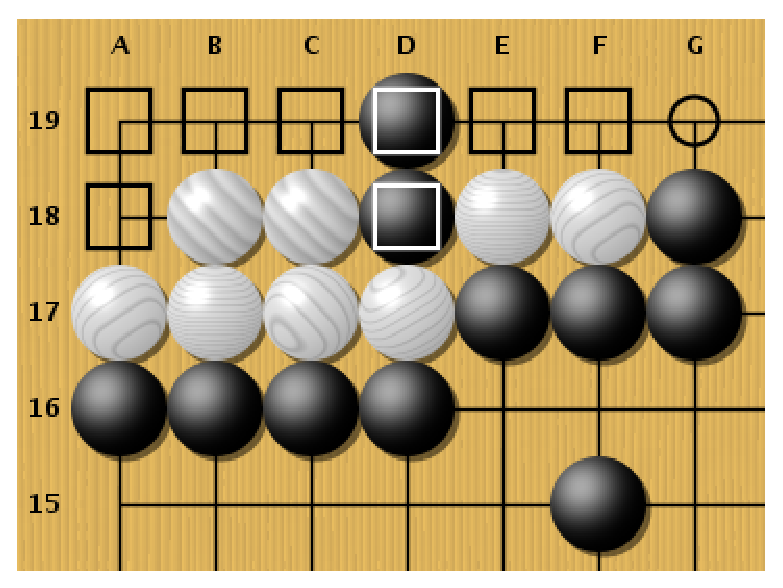
\includegraphics[width = 2.3in]{src/pics/input.eps} 
\caption{Example of input position \label{fig:input}}
\end{center}
\end{figure}

Moreover some comments ( according to sgf format ) might be added to the problem ( in the root node ), these will be included in the output. Example
of input position is shown in Figure~\ref{fig:input}. %together with it's sgf source;


Sgf source of problem given in Figure~\ref{fig:input}:

\begin{verbatim} 
(;GM[1]FF[4]CA[UTF-8]AP[CGoban:2]ST[2]
RU[Japanese]SZ[11]KM[0.00]
CR[ga]AW[bb][cb][eb][fb][ac][bc][cc][dc]
AB[da][db][gb][ec][fc][gc][ad][bd][cd][dd][fe]
SQ[aa][ba][ca][da][ea][fa][ab][db])
\end{verbatim}

\section{Output}

\subsection{Output sgf files} Besides testing messages which are switched off for usual user, program generates short informing messages. Before the
search shows information stored at the problem as comments. After the search informs user of a result of the search, number of searched nodes and time
taken in the search. The most important output of the search are output sgf files. Names of output sgf files is generated from transformed input
position filename ( '/' and '.' are transformed to '\_' ) by adding suffix {\it at.sgf} ( solution with attacker to move ) or {\it de.sgf} ( solution
with defender to move ). In every sgf node there is a short information about depth and status of the node. In nodes where transposition tables cutoff
was performed ( same position in transposition tables was found ) or repetition cutoff was performed ( same position along the path to actual node was
found ) there is a short information about this action. If {\it -to} is switched on node's description are longer containing information about e.g.
potential eyes, possible ko. When {\it -ps} option is switched on, sgf output is pruned to show only relevant information. Thus when attacker moves
first all nodes resulting in the life of the group are pruned and on the other hand when defender moves first all nodes proving the death of the group
are pruned. This restricts the number of nodes a lot and together with marking the output and possible output depth limitation ( option {\it -od}
number ) significantly increases output's legibility. There are three marks used in sgf output: 

\begin{figure}
\begin{center}
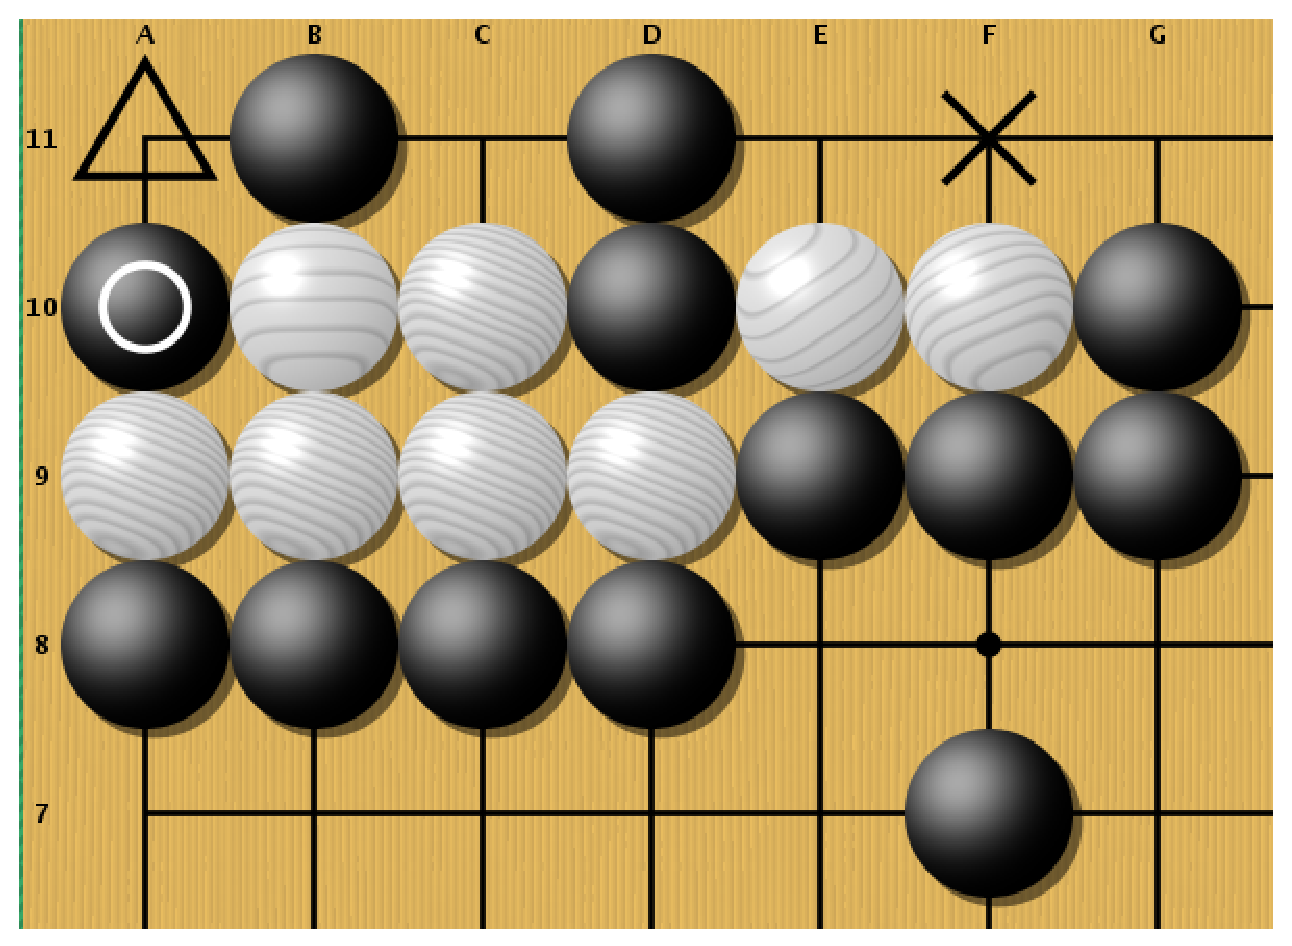
\includegraphics[width=2.3in]{src/pics/output.eps} 
\caption{Position in the sgf output. \label{fig:output}}
\end{center}
\end{figure}

\begin {description}
\item [ Circle ] marks the last played move.
\item [ Cross ] marks the opponent's moves answering last played move.
\item [ Triangle ] marks the coordinate where ko arose in the last turn, therefore opponent cannot play there now.

\end {description}

\noindent Example of position in the single node in the sgf output is shown in Figure~\ref{fig:output}.


